\section{Chính sách dạy: vòng sáu bước và thang gợi ý}\label{sec:policy-design}
Chính sách dạy có hai tầng, cả hai tất định. Tầng trên chọn bài và hoạt động trên đồ thị tri thức theo vòng sáu bước. Tầng dưới điều khiển một câu hỏi từ lúc nêu đến lúc khép, chọn nước đi và bậc gợi ý ở từng lượt. Phần diễn đạt thành lời thuộc về mô hình ngôn ngữ và là phần duy nhất không tất định (mục~\ref{sec:render-design}). Mỗi luật của chính sách có một mã tra cứu trong mã nguồn (dạng \rid{N-*} cho tầng trên và \rid{R-*} cho tầng dưới); mã chỉ để truy vết quyết định và được ghi kèm mỗi quyết định.

\subsection{Vòng sáu bước trên đồ thị}
Gia sư dạy mỗi bài theo sáu bước (Hình~\ref{fig:teaching-loop}). Bước một ôn bài tiên quyết rồi giảng lý thuyết của bài mới, vì học sinh cần nhớ điều đã học trước khi nghe điều mới. Bước hai kiểm tra hiểu bằng một câu hỏi và việc mời học sinh kể lại ý chính. Bước ba đưa ví dụ mẫu rồi một câu cùng làm, trong đó gia sư và học sinh giải chung. Bước bốn luyện tập với độ khó tăng dần, bước năm vận dụng vào tình huống mới, và bước sáu quyết định bài đã qua chưa. Vòng sáu bước là cách đếm của chủ dự án từ ngày 09/11/2026, thay vòng bảy bước trước đó mà không đổi luật điều khiển, giáo án hay công thức mức hiểu; buổi học đã lưu theo vòng cũ vẫn hiển thị đúng nhờ một bảng chuyển.

\begin{figure}[H]
\centering
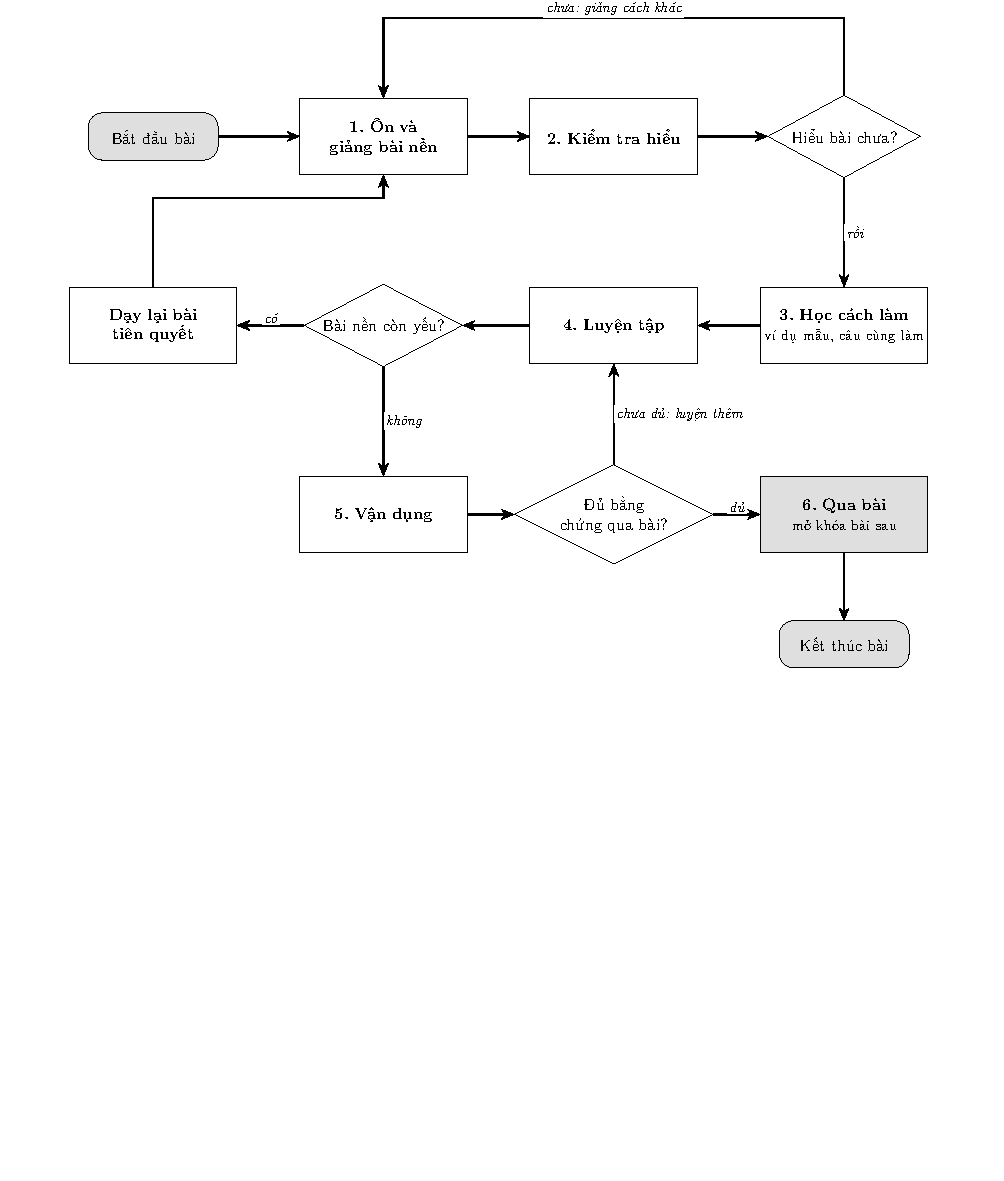
\includegraphics{figures/pdf/fig-teaching-loop.pdf}
\caption{Vòng sáu bước dạy một bài. Hình thoi là các điều kiện do luật của chính sách quyết định; học sinh chưa hiểu thì được giảng cách khác, bài nền còn yếu thì dạy lại bài tiên quyết trước, chưa đủ bằng chứng thì luyện thêm.}
\label{fig:teaching-loop}
\end{figure}

Mười bốn luật tầng trên chạy theo thứ tự ưu tiên và luật đầu tiên có điều kiện thỏa quyết định hành động kế tiếp. Chúng đọc trực tiếp phép chiếu mức hiểu ở mục~\ref{sec:learner-design}. Gia sư tạm dừng bài hiện tại để dạy lại bài tiên quyết khi một lỗi nghiêm trọng thuộc bài tiên quyết, hoặc khi hai lần kiểm tra không qua trong lúc bài tiên quyết còn yếu. Gia sư cho một câu khởi động của bài trước khi vào bài mới mà bài trước chưa có bằng chứng trong buổi, và xen một câu của bài đã qua để ôn lại. Bài được tính là qua khi thỏa quy tắc qua bài (mục~\ref{sec:learner-design}); hết ngân sách câu mà chưa qua thì bài được ghi là cần học lại.

\subsection{Thang gợi ý từ H0 đến H7}
Trong một câu hỏi, sự trợ giúp được lượng hóa bằng thang tám bậc từ H0 (không gợi ý) đến H7 (giải thích đầy đủ), theo hai trục: bậc là bao nhiêu trợ giúp, mục tiêu là trợ giúp nhắm vào đâu (đề bài, khái niệm, chiến lược, bước làm, cách viết đáp số hoặc việc tự kiểm tra). Bảng~\ref{tab:ladder} nêu tám bậc với ví dụ cho câu ``viết phân số $9/10$ dưới dạng số thập phân'' (đáp án $0{,}9$). Mỗi bậc có một trọng số độc lập $\iota_h$ do khung đánh giá quy định, được mô hình người học dùng ở mục~\ref{sec:learner-design}, nên gia sư và bộ đánh giá nói cùng một ngôn ngữ về mức học sinh đã được giúp.

\begin{table}[H]
\centering
\caption{Thang gợi ý. Trọng số $\iota_3$ và $\iota_5$ là diễn giải khai báo (DI) nội suy giữa các giá trị của khung đánh giá.}\label{tab:ladder}
\small
\begin{tabular}{>{\raggedright\arraybackslash}p{0.9cm}>{\raggedright\arraybackslash}p{2.9cm}>{\raggedright\arraybackslash}p{8.4cm}r}
\toprule
Bậc & Tên & Ví dụ & $\iota_h$ \\
\midrule
H0 & không gợi ý & --- & $1{,}00$ \\
H1 & câu hỏi định hướng & ``Mình cần viết $9/10$ thành số thập phân. Con đọc phân số này giúp cô nhé?'' & $0{,}85$ \\
H2 & nhắc khái niệm & ``Mẫu số 10 cho biết phần thập phân có mấy chữ số?'' & $0{,}70$ \\
H3 & gợi ý chiến lược & ``Con thử viết chữ số 9 vào hàng phần mười xem sao?'' & $0{,}60$ \\
H4 & cho một bước trung gian & ``Phần nguyên là 0, hàng phần mười là chữ số 9. Vậy viết thế nào?'' & $0{,}50$ \\
H5 & chia nhỏ bài & ``Mình làm từng bước nhỏ. Mẫu số của $9/10$ là bao nhiêu?'' & $0{,}35$ \\
H6 & cùng làm từng bước & Trình bày các bước, học sinh làm bước cuối & $0{,}20$ \\
H7 & giải thích đầy đủ & Giải thích như lời giải mẫu rồi mời trình bày lại & $0{,}00$ \\
\bottomrule
\end{tabular}
\end{table}

Mỗi câu luyện tập mang thang gợi ý riêng: các bậc H1 đến H3 do giáo viên duyệt, các bậc cao hơn rút từ lời giải, và khi câu thiếu một bậc thì gợi ý chung của bài thay vào. Thang không bao giờ tự nói đáp án; chỉ bậc H7 được phép nói đáp án và chỉ ở hoạt động luyện tập. Trong bài kiểm tra, bậc gợi ý bị chặn ở H1 và câu vượt trần được khép với trạng thái chưa giải được.

\subsection{Chính sách của vòng một câu hỏi}
Vòng một câu hỏi là một máy trạng thái chạy từ lúc nêu câu đến khi khép câu. Mỗi tin nhắn của học sinh được bộ đọc phân loại thành lần thử có thể chấm, xin gợi ý, đòi đáp án, hỏi lại đề, hỏi nghĩa một từ, lạc đề hoặc cảm xúc tiêu cực, rồi hợp vào trạng thái của câu và đưa cho hàm quyết định. Hàm này là danh sách luật có thứ tự: luật đầu tiên thỏa điều kiện quyết định nước đi, bậc và mục tiêu, và mã luật được ghi vào sổ cùng quyết định, nên mỗi hành vi của gia sư giải thích và kiểm thử được theo từng luật. Phiên bản hiện hành có $29$ luật; Bảng~\ref{tab:rules} nêu các họ chính.

{\small
\begin{longtable}{>{\raggedright\arraybackslash}p{3.3cm}>{\raggedright\arraybackslash}p{5.4cm}>{\raggedright\arraybackslash}p{6.0cm}}
\caption{Các họ luật chính của vòng một câu hỏi.}\label{tab:rules}\\
\toprule
Luật & Điều kiện & Quyết định \\
\midrule
\endfirsthead
\toprule
Luật & Điều kiện & Quyết định \\
\midrule
\endhead
\bottomrule
\endfoot
\rid{R-FIRST-WRONG} & Câu sai đầu tiên, chưa có gợi ý & Hỏi ``con đã làm thế nào''; chưa gợi ý \\
\rid{R-SLIP} & Lỗi tính toán, phương pháp đúng & Gợi ý H1, mục tiêu tự kiểm tra \\
\rid{R-MISC-HIGH} & Nhận ra lỗi quan niệm với độ tin cậy từ $0{,}7$ & Gợi ý từ H2 về khái niệm; đưa phản ví dụ khi có \\
\rid{R-LADDER}, \rid{R-ESCALATE} & Sai các lần sau; sai lặp lại cùng mục tiêu & Bậc không thấp hơn bậc đã dùng; thêm một bậc, hai bậc khi có dấu hiệu nản \\
\rid{R-DEESCALATE} & Một bước đúng sau gợi ý & Hạ một bậc, giảm dần giàn giáo \\
\rid{R-HELP-REQUEST} & Xin gợi ý, ``con không biết'', đòi đáp án & Đề nghị chọn một lần, rồi gợi ý kế tiếp; đòi đáp án thì từ chối nhẹ và gợi ý \\
\rid{R-OFF-TOPIC}, \rid{R-CLARIFY}, \rid{R-AFFECT} & Lạc đề; ``là sao ạ''; ``chán quá'' & Kéo về câu; nói lại đề; công nhận cảm xúc rồi gợi ý. Không tính là sai \\
\rid{R-FRUSTRATION}, \rid{R-FULL} & Ba lượt không tiến bộ hoặc quá $300$ giây; cùng làm vẫn không tiến & Cùng làm từng bước (H6); giải thích đầy đủ (H7, chỉ khi luyện tập), rồi mời giảng lại \\
\rid{R-VERIFY} & Trả lời đúng và thuộc diện cần xác nhận (DI) & Hỏi ``vì sao'' \\
\rid{R-ASSESS-CAP} & Câu của bài kiểm tra & Bậc tối đa H1; quá thì khép câu \\
\end{longtable}}

Chính sách không dùng số ngẫu nhiên: việc chọn câu đúng nào để hỏi ``vì sao'' dùng giá trị băm của mã câu, nên cùng một buổi học luôn cho cùng một quyết định và phát lại được. Những lượt không phải một lần thử, như lạc đề hay ``là sao ạ'', không bị tính là sai vì chấm một lời than thở là sai sẽ phạt học sinh vì điều em không làm. Câu đúng từng phần không làm tăng bậc gợi ý, và câu đúng sau giải thích đầy đủ không bao giờ được tính là thành công của bài.
